%sri
\section{Introduction}

A failure during a large-scale execution of any application on an extreme-scale
system leads to loss of time and money, and can cause a nightmare to any
application developer. While failures could be due to application bugs,
failures due to errors not detectable by error correcting code (ECC) are on the
rise.  For example, Geist states that such failures are a common occurrence on
Oak Ridge National Laboratories leadership class machines~\cite{errors_ecc},
and Schroeder and Gibson state that a large number of CPU and memory failures
were from parity errors after tracking a five-year log of hardware replacements
for a $765$ node high-performance computing cluster~\cite{schroeder_gibson}.
Echoing the sentiment of Snir et al.~\cite{snir}, we believe it is critical to
overcome the effect of such failures through a productive and performant resilience 
interface in the parallel programming model so that a developer can make avail 
the performance on extreme- and upcoming exa-scale parallel systems.

The traditional solutions to address failures during large-scale parallel
executions includes the application developer: (a) manually takes periodic
checkpoints, and manually controls the rollback and restart from specific
checkpoints~\cite{checkpointrestart}, (b) employs a semi-automatic approach, 
where the developer employs programming constructs that have well defined 
semantics in the event of failures, e.g, \texttt{finish} blocks in X10~\cite{X10}.
Here, the parallel programming model runtime automatically corrects itself to 
handle further execution in the event of a failure but limited to the beginning
of these specific programming constructs. (c) employs a sophistica

In x10, use programming language constructs such as resilient finish blocks to
capture their completing along with useful semnatic guarantees. 

Autocorrecting, where the programmer labels computations which form. 

We believe these solutions are good, but not flexible to demand the
complexities of current extreme-scale and upcoming exa-scale systems. Its is
not at one point, every mapping needs to make a decision, support for checking
whther there is a tradeoff between recomputing the dag vs .. this has to be
dynamic. We also believe that these decision should be in a deferred execution
state, not the whole computation stopping.


To drive this point, consider the figure . A simple computation task graph, X10
would allow this, PARSEC would allow this, Charm++ would focus on the stores of
alpha, x and y. However, we believe that this solution.  soemtimes you have a
resilient store where you map alpha, x but sometimes not. Think here.

The right vehicle to demonstrate such a dynamic decision for checkpoints, along
with a deferred execution model is the Legion programming model. The strengths
of this include a decoupled scheduling, mapping, and execution analysis stages
that drives this solution.

\begin{figure}
\centering
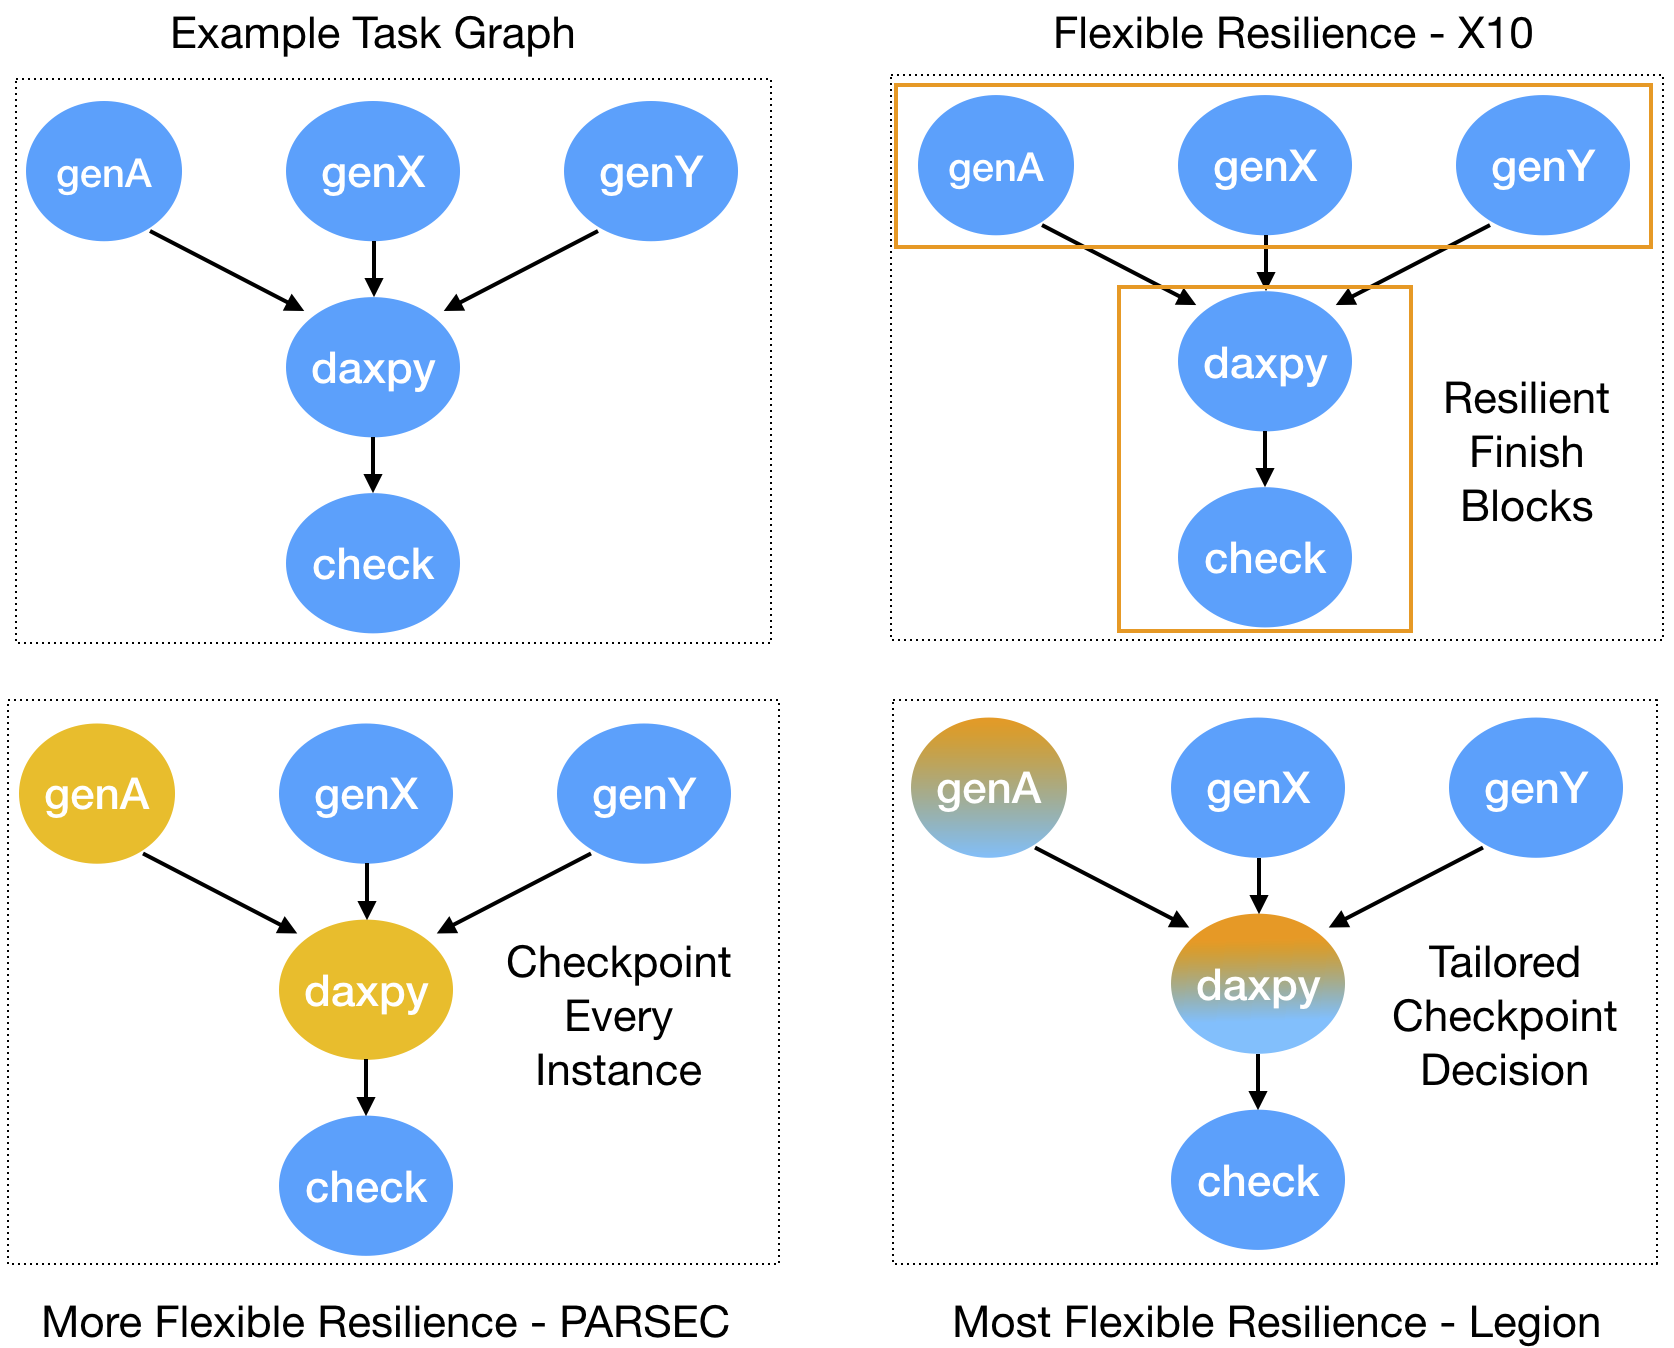
\includegraphics[width=.42\textwidth]{images/spectrum_x10_parsec_legion_policies.png}
\caption{A spectrum of resilience mechanism supported by different
state-of-the-art parallel runtimes along with the proposed resilience strategy
for Legion.} 
\end{figure}

Our contributions are as follows: 
\begin{itemize} 
\item the most flexible resilience mechanism 
\item dynamic decisions for checkpointing 
\item auto rollback and recovery 
\item garbage collector that will also collect previous 
checkpoints based on a novel post-dominator algorithm.  
\item a discussion of the semantics of regions when there is rollback 
\end{itemize}

The rest of the paper is organized as follows:

%With the advent of productive programming models like Legion~\cite{legion},
%X10~\cite{x10}, PARSEC~\cite{parsec}, CHARM++~\cite{charm++}, and others,
%programming extreme-scale systems is not as significant a challenge as
%addressing other 
%
%how is it different from x10, parsec, charm++\\
%	- they also allow tasks to be marked as resilience\\
%	- x10 allows finish blocks, exception semantics.\\
%	- what are the exception semantics that we are providing\\
%
%what about local vs global recovery\\
%	- can we recover from a node failure\\
%	- can we recover from an exception, what are the semantics that we provide
%	  here\\
%	- can we recover from ECC errors, \\
%	- can we fix these errors ?\\
%	- can we recover from I/O errors ?\\ 
%	- can we recover from non-SingleTasks, what is recovery for index space
%	  tasks, must epoch tasks\\
%
%
%experiments: circuit, miniAero, Soleil-X, stencil, (S3D ?)\\
%
